\documentclass{beamer}
\usepackage[utf8]{inputenc}
\usepackage[spanish]{babel}
\usepackage{graphicx}
\usepackage{caption}
\usepackage{refstyle}
\usepackage{blindtext}
\usetheme{Madrid}
\hypersetup{
  colorlinks=true,
  linkcolor=blue!50!red,
  urlcolor=green!70!black
}

\begin{document}

\title{Docking molecular de la proteína E del SARS-CoV-2 y la amantadina}

\subtitle{Doctorado en Investigaciones Cerebrales \\ Instituto de Investigaciones Cerebrales \\Universidad Veracruzana}
\author{M. en NE. Rodrigo Ramírez Rodríguez}
\date{\today} 

\begin{frame}
\titlepage
\end{frame}

\begin{frame}
\frametitle{Introducción}
\begin{itemize}
    \item El virus del SARS-CoV-2 ha impactado la salud mundial, en particular, afectando las funciones respiratorias (Mohanty et al., 2020). 
    \item Se han propuesto fármacos para reducir la sintomatología de este virus pero basado en hipótesis (Lai et al., 2020).
    \item La proteína E de este virus se encarga de la generación de viroporinas las cuales son canales creados en la célula del hospedero que facilitan la diseminación del virus (Naqvi et al., 2020).
    \item Un estudio de docking reciente indica que la amantadina puede interactuar con puentes de hidrógeno con los aminoácidos fenilalanina 26 y alanina 22 (Aranda-Abreu et al., 2020)
\end{itemize} 

   
 
\end{frame}

%

\begin{frame}{Problema a resolver}
\begin{itemize}
    \item Dado que el modelo de la proteína E contiene diversos modelos, esta investigación tuvo como objetivo realizar docking molecular de un modelo estructural de la proteína E usando como ligando a la amantadina.
    \item La proteína E (7K3G) se adquirió de Protein Data Bank y la amantadina (DB00915) se adquirió de DrugBank Online.
    \item Mediante Autodock y Autodock Vina se determinaron cualés son los aminoácidos con los que la amantadina interacciona con el dominio de transmembrana hidrofóbico de la proteína E y su respectiva energía de afinidad.
    
\end{itemize}  
  
    
\end{frame}


%

\begin{frame}{Resultados}

%\begin{itemize}
    %\item 

El docking, con la semilla aleatoria -834651280, se obtuvieron nueve conformaciones del ligando DB00915 (Figura \ref{dock}).
    
    
    
\begin{figure}
    \centering
    \includegraphics[width=0.50\textwidth]{Dockeo.png}
    \caption{Conformaciones de DB00915 con la proteína E del SARS-CoV-2}
    \label{dock}
\end{figure}     
    
    
    
\end{frame}    
    
    
    
    
\begin{frame}    
    
El modo 1 indica una alta energía de afinidad de -5.5 (kcal/mol)(Figura \ref{afinidad}).
   
 \begin{figure}
    \centering
    \includegraphics[width=0.60\textwidth]{conformación 1.png}
    \caption{Conformación 1 de DB00915 con la proteína E del SARS-Cov-2}
    \label{afinidad}
\end{figure} 
  
%\end{itemize}

\end{frame}



\begin{frame}{Resultados}
Vina indica que el DB00915 interacciona con la proteína E mediante la unión con puentes de hidrógeno  de los aminoácidos Leucina 18 y Asparagina 15 (Figura \ref{amino}).

\begin{figure}
    \centering
    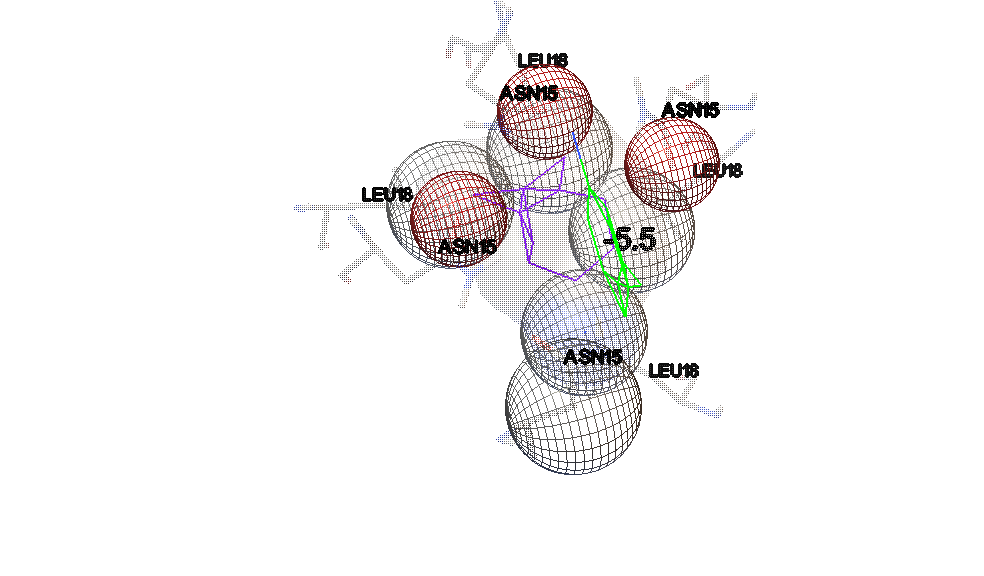
\includegraphics[width=0.60\textwidth]{Docking Protein E - amantadina.png}
    \caption{Interacción de los aminoácidos LEU 18 y ASN 15 en la conformación 1 de DB00915 con la proteína E del SARS-CoV-2}
    \label{amino}
\end{figure} 


\end{frame}





\begin{frame}{Conclusiones}
\begin{itemize}
    \item La amantadina ha mostrado tener sitios de unión con la proteína E del SARS-Cov-2 en los aminoácidos alanina 22 y fenilalanina 26 (Aranda-Abreu et al., 2020).
    \item Los resultados de este experimento por docking indican que la amantadina tiene otros sitios de unión en los aminoácidos LEU 18 y ASN 15. Esto sugiere que la amantadina puede actuar en diversos puntos de unión de la proteína E reduciendo su capacidad para formar viroporinas.
    \item Estos datos apoyan el uso de la amantadina como un potencial fármaco para mitigar los efectos del SARS-CoV-2.
\end{itemize}

\end{frame}

\begin{frame}{Referencias}
\begin{itemize}
    \item Aranda-Abreu, G. E., Hernández-Aguilar, M. E., Herrera-Covarrubias, D. y Rojas-Durán, F. (2020). Amantadine as a drug to mitigate the effects of COVID-19. Medical Hypothesis. https://doi.org/10.1016/j.mehy.2020.109755
    
    \item Mohanty, S. K., Satapathy, A., Naidu, M. M., Mukhopadhyay, S., Sharma, S., Barton, L. M., Stroberg, E., Duval, E. J., Pradhan, D., Tzankov, A. y Parwani, A. V. (2020). Severe acute respiratory syndrome coronavirus-2 (SARS-CoV-2) and coronavirus disease 19 (COVID-19) - anatomic pathology perspective on current knowledge. Diagnostic Pathology.
https://doi.org/10.11862Fs13000-020-01017-8
\end{itemize}

\end{frame}

\begin{frame}{Referencias}
    
\begin{itemize}
\item Naqvi, A. A. T., Fatima, K., Mohammad, T., Fatima, U., Singh, I. K., Singh, A., Atif, S. M., Hariprasad, G., Hasan, G. M. y Hassan, M. I. (2020). Insights into SARS-CoV-2 genome, structure, evolution, pathogenesis and therapies: structural genomics approach. Biochimica et Biophsyca Acta Molecular Basis of Disease. https://doi.org/10.1016/j.bbadis.2020.165878

\item Lai,C-C., Shih, T-P., Ko, W-C., Tang, H-J. y Hsueh, P-R. (2020). 
Severe acute respiratory syndrome coronavirus 2 (SARS-CoV-2) and coronavirus disease-2019 (COVID-19): the epidemic and the challenges. 
International Journal of Antimicrobial Agents.
https://doi.org/10.10162Fj.ijantimicag.2020.105924
    
\end{itemize}
\end{frame}

\end{document}
